\documentclass{llncs}

\usepackage{amsmath}
\usepackage{amsfonts}
\usepackage{amssymb}
\usepackage{xspace}
\pagestyle{plain}
\usepackage{algorithm,algpseudocode}
\usepackage{caption}
\usepackage{subcaption}
\captionsetup{compatibility=false}
\usepackage{mathtools}
\usepackage{tikz}
\usepackage{url}
\usetikzlibrary{arrows,calc}


\newcommand{\hide}[1]{}

\newcommand{\valueof}[1]{[\![{#1}]\!]}

\newcommand{\bbfR}{\mathbb{R}}
\newcommand{\bbfS}{\mathbb{S}}
\newcommand{\bbfD}{\mathbb{D}}
\newcommand{\bbfRU}{\mathbb{R}^{[0, 1]}}
\newcommand{\calM}{\mathcal{M}}
\newcommand{\od}{\overline{\mathbf{d}}}
\newcommand{\oD}{\overline{\mathbf{D}}}
\newcommand{\Act}{\Sigma}
\newcommand{\Obs}{\Omega}
\newcommand{\obs}{\omega}
\newcommand{\Info}{\Theta}
\newcommand{\info}{\theta}
\newcommand{\sch}[1]{\mathfrak{#1}}

\newcommand{\AP}{\mathit{AP}}
\newcommand{\X}{\mathsf{X}\xspace}
\newcommand{\F}{\mathsf{F}\xspace}
\newcommand{\G}{\mathsf{G}\xspace}
\newcommand{\until}{\mathbin{\mathsf{U}}}
\newcommand{\PCTL}{\textsf{PCTL}\xspace}
\newcommand{\PJ}[1]{\mathbb{P}_{#1}}
\newcommand{\scheduler}[1]{\mathfrak{#1}}
\newcommand{\myPr}[3]{{\Pr}^{#2}({#1}, {#3})}
\newcommand{\dpriv}[2]{\mathcal{D}_{{#1}, {#2}}}
\newcommand{\myE}[3]{\mathbb{E}_{#1}({#2}, {#3})}
\newcommand{\zpython}{\textsc{Z3Python}\xspace}

\algnewcommand\algorithmicmatch{\textbf{match}}
\algnewcommand\algorithmicwith{\textbf{with}}
\algnewcommand\algorithmiccase{\textbf{case}}
% New "environments"
\algdef{SE}[MATCH]{Match}{EndMatch}[1]{\algorithmicmatch\ {#1}\ \algorithmicwith}{\algorithmicend\ \algorithmicmatch}%
\algdef{SE}[CASE]{Case}{EndCase}[1]{\algorithmiccase\ {#1}:}{\algorithmicend\ \algorithmiccase}%
\algtext*{EndMatch}%
\algtext*{EndCase}%
\algnewcommand{\IfThenElse}[3]{% \IfThenElse{<if>}{<then>}{<else>}
  \State \algorithmicif\ #1\ \algorithmicthen\ #2\ \algorithmicelse\ #3}
\newcommand{\lCase}[2]{\State \textbf{case} {#1}{:} {#2}}


\title{Partially Observable Markov Decision Processes}

\begin{document}

\maketitle

\begin{abstract}
  Use POMDP to formalize privacy
\end{abstract}

\section{Introduction}
\label{section:introduction}

% importance of privacy and its formal analysis

Privacy has been a hotly debated issue since late nineteenth
century~\cite{WB:90:RP}. With the advent of social media, privacy is
perhaps one of the most relevant topics in the digital age as
well. Indeed, numerous privacy measures for publishing data
have been proposed~\cite{S:2002:KAMPP,FWC:10:PPDP}. Whether these
measures are taken properly and effectively concerns every
individuals. The importance of privacy research is thus noted by the
formal method community as well~\cite{TW:09:FMP}.

% differential privacy

Differential privacy is a framework for the design of privacy
measures~\cite{D:06:DP,DR:14:AFDP}. In the framework, data publishing
mechanisms are formalized as randomized algorithms. On any input data
set, such mechanisms return randomized answers to data users' queries.
Output distributions naturally correspond to information released by
data publishing mechanisms. In order to preserve privacy, data
curators suffice to ensure that similar output distributions are
yielded by mechanisms on similar input data sets. Thanks to its simple
formalization, differential privacy moreover allows data curators
to evaluate privacy and utility quantitatively. The framework
subsequently attracts lots of attentions from academia and industry.

% pufferfish privacy

Pufferfish is a more recent privacy framework which subsumes
differential privacy~\cite{KM:14:PFMPD}. In differential privacy,
there cannot be correlation among entries in data sets. For data sets
with correlated entries, differential privacy can still leak
noticable private information~\cite{KM:11:NFLDP}. The no free lunch
theorem in data privacy shows that prior knowledge about data sets is
crucial to privacy analysis. The Pufferfish privacy framework allows
data curators to analyze privacy with prior knowledge about data
sets. Under the Bayesian privacy framework, it is shown that
differential privacy preserves privacy if there is no correlation
among entries in data sets (Theorem~2 in~\cite{KM:14:PFMPD}).

% importance of formal methods in privacy

Although privacy frameworks help data curators design data publishing
mechanisms, they do not necessarily induce privacy-respecting
mechanisms. In differential and Pufferfish privacy, data publishing
mechanisms are analyzed with sophisticated mathematical tools.
Misinterpretation of privacy proofs can lead to incorrect
modifications or generalizations of privacy-respecting mechanisms.
Indeed, several published variations of differentially private
mechanisms are shown to voilate privacy~\cite{DWWZK:18:DVDP}. The
formal method community has also started to develop techniques for
checking differentially private
mechanisms~\cite{TKD:11:FVDPIS,GHHNP:13:LDTDP,BDGKZ:13:VCDP}.

% markov models as formal models for privacy analysis
% hidden markov models

In this work, we focus on a lightweight but automatic technique for
checking Pufferfish privacy. Our goal is to develop a general
verification technique for the Bayesian privacy framework. To do so,
we propose a formal model for data publishing mechanisms and
investigate the verification problem for Pufferfish privacy.
In~\cite{LWZ:18:MCDPP}, the authors propose Markov chains and Markov
decision processes to model data publishing mechanisms. Several known
mechanisms are formalized as different Markov models and checked to
satisfy differential privacy.

We propose to formalize Pufferfish privacy on hidden Markov models. A
data publishing mechanism is again the underlying Markov
chain associated with a hidden Markov model. Attackers' prior
knowledge is thus modeled by an initial state distribution. Based on
our formalization, we give a formal model for the geometric mechanism
and analyze it with Pufferfish privacy. Interestingly, hidden Markov
models allow us to explain subtleties between differential privacy and
Pufferfish privacy concisely. This strongly favors our formalization
as the right abstraction for Pufferfish privacy. We believe data
curators will be able to understand the Bayesian privacy framework
through this work.

We furthermore investigate the verification problem for Pufferfish
privacy on hidden Markov models. By showing the reduction from the
Boolean Satisfiability Problem(SAT), the verification problem proves
to be NP-hard. Though, using Satisfiability Modulo Theories solvers,
we design a verification algorithm and automatically verify Pufferfish
privacy problems with our implementation in \zpython.

The rest of the paper is organized as follows. Preliminaries are given in
Section~\ref{section:preliminaries}. In Section~\ref{section:pufferfish}
and Section~\ref{section:hmm}, we discuss Pufferfish privacy framework
and several privacy examples modeling in HMMs. In Section~\ref{section:complexity}
and Section~\ref{section:checking-pufferfish}, we investigate the complexity
of verification problem in Pufferfish and design an automatic algorithm
to verify it. A classical case study is given in Section~\ref{section:noisy-max}
and conclusions are discussed in Section~\ref{section:conclusions}.

% results



\section{Preliminaries}
\label{section:preliminaries}

A \emph{Markov decision process (MDP)} $M = (\Act, S, p, L)$ consists of
a finite set $\Act$ of \emph{actions}, a set $S$ of \emph{states}, a
\emph{labelling function} $L : S \rightarrow 2^{\AP}$, and 
a \emph{transition distribution} $p : \Act \times S \times S
\rightarrow \bbfRU$ such that $\sum_{t \in S} p (s, a, t) = 1$
for every $a \in \Act$ and $s \in S$. If the set of states is finite,
we say $M$ is a \emph{finite} MDP.

A \emph{partially observable Markov decision process (POMDP)} $P =
(M, \Obs, r)$ is a finite MDP $M = (\Act, S, p, L)$ with a finite set
$\Obs$ of \emph{observations} and an \emph{observation distribution} $o
: \Act  \times S \times \Obs \rightarrow \bbfRU$ such that $\sum_{\obs
  \in \Obs} o (a, s, \obs) = 1$ for every $a \in \Act$ and $s \in S$.
A POMDP models an MDP with incomplete information. The current state
of the underlying MDP is not known precisely. Rather, schedules are
made by observations and state distributions. 

Formally, let $\Info (S) = \{ \info \in S \rightarrow \bbfRU : \sum_{s \in
 S} \info (s) = 1 \}$ be the set of probability distributions on $S$. 
Consider an \emph{initial state distribution} $\info_0 \in \Info (S)$. A
\emph{history} $H_i$ up to time $i$ is a sequence $\info_0, a_1, \obs_1,
a_2, \obs_2, \ldots, a_{i-1}, \obs_{i-1}$. At time $i$, $H_i$ is the
only information available externally. If an action $a_i$ is chosen
at time $i$ based on $H_i$, the following steps are carried out
consecutively:
\begin{enumerate}
\item If the current state is $s_{i-1}$, the POMDP moves to the state
  $s_i$ with probability $p (s_{i-1}, a_i, s_i)$;
\item An observation $\obs_i$ is received with probability $o (a_i, s_i,
  \obs_i)$; and
\item The history $H_{i+1}$ becomes $H_i, a_i, \obs_i$.
\end{enumerate}
Note that histories do not contain states but the underlying MDP
updates its state as usual. Based on this formalization, we can now
define schedulers for POMDP. Let $\Xi$ be the set of histories. A
\emph{scheduler} $\sch{S} : \Xi \rightarrow \Act$ for the POMDP $P
= (M, \Obs, w)$ with $M = (\Act, S, p, L)$ is a function
from histories to actions. 

Interestingly, it is not necessary to keep
histories. For schedulers, it suffices to maintain the current state
distribution. Let $\info \in \Info (S)$ be a state distribution. Define
$T (\info, a, \obs) \in \Info (S)$ by
\begin{eqnarray}
  \Pr(\obs | \info, a) & = &
    \sum_{s, t \in S} \info (s) p (s, a, t) o (a, t, \obs)
\label{eqn:state-distribution-observation}
\\                             
  T (\info, a, \obs) (t) & = &
    \frac{\sum_{s \in S} \info (s) p (s, a, t) o (a, t, \obs)}
         {\Pr (\obs | \info, a)}.
\label{eqn:state-distribution-successor}
\end{eqnarray}
That is, $T (\info, a, \obs)$ is the posterior state distribution given
the prior state distribution $\info$, action $a$, and observation
$\obs$. Now recall that the initial state distribution $\info_0$ is
known. Let $\info_{i-1} \in \Info (S)$ be the state distribution at
time $i - 1$. Suppose a scheduler takes the action $a_{i}$ and
observes $\obs_{i}$ at time $i$. Then $\info_i = T (\info_{i-1}, a_i,
\obs_i)$ is the state distribution at time $i$. A
scheduler can then decide the next action $a_{i+1}$ by $\info_i$
accordingly. 

Let $R (s, a)$ be the reward for the state $s$ on the action
$a$, and $\overline{R} (s)$ be the reward for terminating at the state
$s$.\footnote{Observe that $R (s, a)$ is received when the MDP
\emph{leaves} $s$.} For $0 \leq \beta \leq 1$, the scheduler attaining
the maximal expected reward
\[
  E[\beta^T \overline{R} (s_T) + \sum_{i=0}^{T-1} \beta^i R(s_i, a_{i+1})]
\]
can be obtained by iteration. Let $L_{< \infty} (\Info (S))$ be the set of
bounded real-valued functions on $\Info (S)$. Consider
$\Upsilon : \Info (S) \times \Act \times L_{< \infty} (\Info (S)) \rightarrow
\bbfR$ defined by
\[
  \Upsilon (\info, a, f) = \sum_s \info (s) R (s, a) +
  \beta \sum_{\obs \in \Obs}
  \sum_{s, t \in S} \info (s) p (s, a, t) o (a, t, \obs) f (T (\info, a, \obs)).
\]
For $\info \in \Info (S)$, define
\begin{eqnarray}
  \overline{V}_{T} (\info) & = & \sum_s \info (s) \overline{R} (s)
\label{eqn:terminate-probability}
\\
  \overline{V}_{i} (\info) & = &
    \max_{a \in \Act} \{ \Upsilon (\info, a, \overline{V}_{i+1}) \} 
    \hspace{2em} (0 \leq i < T)
\label{eqn:max-probability}
\end{eqnarray}

It is more convenient to use matrices to simplify various
expressions. Without loss of generality, assume $S = \{ 1, 2, \ldots,
n \}$ when $|S| = n$. A state distribution $\info \in \Info (S)$ is
represented by the column vector $(\info (1), \info (2), \ldots, \info
(n))^T$  where $v^T$ is the transpose of the vector $v$.
For $a \in \Act$, let $P^a = [p_{ij}^a]_{|S|
  \times |S|}$ denote the transition matrix where $p_{ij}^a = p (i, a,
j)$. For $a \in \Act, \obs \in \Obs$, let $O^a (\obs) = [
o^a_{ij} ]_{|S| \times |S|}$ be the diagonal matrix where
\begin{eqnarray*}
  o^a_{ij} & = & \left\{
                 \begin{array}{ll}
                   o (a, i, \obs) & \textmd{ if } i = j\\
                   0 & \textmd{ otherwise}
                 \end{array}
                 \right.
\end{eqnarray*}
Let $e$ be the $n$-column vector whose entries are $1$.
Then $(\ref{eqn:state-distribution-observation})$ and
$(\ref{eqn:state-distribution-successor})$ rewrite to
\begin{eqnarray}
  \Pr (\obs | \info, a) & = & \info^T P^a O^a (\obs) e \\
  T (\info, a, \obs) & = & \frac{\info^T P^a O^a (\obs)}
                                {\Pr (\obs | \info, a)}
\end{eqnarray}
Similarly, let $R^a = (R (a, 1), R (a, 2), \ldots, R (a, n))^T$ be the
vector of rewards associated with the actcion
$a$. Equations~$(\ref{eqn:terminate-probability})$ and 
$(\ref{eqn:max-probability})$ rewrite to 
\begin{eqnarray}
  \overline{V}_{T} (\info) & = & \info^T \overline{R}\\
  \overline{V}_i (\info) & = &
        \max_{a \in \Act} \left\{ \info^T [
        R^a + 
        \beta \sum_{\obs \in \Obs}
          P^a O^a (\obs) \overline{V}_{i+1} ] \right\}
          \hspace{2em}(0 \leq i < T)
\end{eqnarray}

\hide{
\begin{eqnarray*}
  \overline{V}_{T} (\info) & = & \info^T \overline{R}\\
  \overline{V}_i (\info) & = &
        \max_{a \in \Act} \left\{ \info^T [
        R^a + 
        \beta \sum_{\obs \in \Obs} P^a O^a (\obs) \gamma^{l (\info, a,
                               \obs, i + 1)} ] \right\}\\
  l (\info, a, \obs, i) & = &
      \max_{\gamma \in \Gamma_{i}}
        \{ \info^T P^a O^a (\obs) \gamma \}
\end{eqnarray*}
}

\section{Pufferfish Privacy Framework}
\label{section:pufferfish}

Differential privacy is a privacy framework for design and analysis of
data publishing mechanisms~\cite{D:06:DP,DR:14:AFDP}. In the
framework, a \emph{data set} is an
ordered collection of \emph{data entries}. Two data sets $\od$ and
$\od'$ are \emph{neighbors} (written $\Delta (\od, \od') \leq 1$) if
$\od$ and $\od'$ are identical except for one data entry. A \emph{data
publishing mechanism} (or simply \emph{mechanism}) $\calM$ is a
randomized algorithm which takes a data set $\od$ as inputs. A
mechanism satisfies $\epsilon$-differential privacy if its output
distributions differ by the multiplicative factor $e^\epsilon$  at
most on
every neighboring data sets.

\begin{definition}
  Let $\epsilon > 0$. A mechanism $\calM$ is
  \emph{$\epsilon$-differentially private} if for all $r \in
  \textmd{range}(\calM)$ and data sets $\od, \od'$ with $\Delta (\od,
  \od') \leq 1$, we have
  \[
    \Pr (\calM (\od) = r) \leq e^{\epsilon} \Pr (\calM (\od') = r).
  \]
\end{definition}

For any data entry $d$ in a data
set $\od$, consider the data set $\od'$ obtained by removing $d$ from
$\od$. Then $\Delta (\od, \od') \leq 1$. For any
$\epsilon$-differentially private mechanism $\calM$, we have
$e^{-\epsilon} \Pr (\calM (\od') = r) \leq \Pr (\calM (\od) = r)
\leq e^{\epsilon} \Pr (\calM (\od') = r)$ for every $r$. That is, the
probabilities of observing $r$ are bounded by the multiplicative
factor $e^{\epsilon}$ when the data entry $d$ is present or absent.
Intuitively, $\epsilon$-differential privacy ensures similar output
distributions on similar data sets. Limited information about each
data entry is revealed. Individual privacy is hence preserved.

Differential privacy implicitly assumes each data entry is
independent. For data sets with correlated data entries, differential
privacy may reveal too much information about individuals. Consider,
for instance, a data set of family members. If a family member has
contracted a (very) contagious disease, all members are likely to have
the same disease. In order to decide whether a specific family member
has contracted the disease, it suffices to determine whether
\emph{any} family member has the disease. It appears that global
information can be inferred from any differential information
when data entries are correlated. Differential privacy may be
insufficient to preserve privacy~\cite{KM:11:NFLDP}.

Pufferfish is a Bayesian privacy framework which subsumes differential
privacy~\cite{KM:14:PFMPD}. In Pufferfish privacy, a random variable
$\oD$ represents a data set drawn from a distribution $\theta \in
\bbfD$. The set $\bbfD$ of distributions formalizes prior knowledge
about data sets, such as whether data entries are independent or
correlated. Moreover, a set $\bbfS$ of \emph{secrets} and
a set $\bbfS_{\textmd{pairs}} \subseteq \bbfS \times \bbfS$ of
\emph{discriminative secret pairs} formalize the information to be
protected. Consider a pair $(s_i, s_j)$ of discriminative secrets and
a data set $\oD$ drawn from $\theta \in \bbfD$. A mechanism $\calM$
satisfies $\epsilon$-Pufferfish privacy if its output distributions
differ by at most the multiplicative factor $e^{\epsilon}$ when
conditioned on the secrets $s_i$ and $s_j$.

\begin{definition}
  Let $\bbfS$ be a set of secrets, $\bbfS_{\textmd{pairs}}$ a set of
  discriminative secret pairs, $\bbfD$ a set of data evolution
  scenarios, and $\epsilon > 0$, a mechanism $\calM$ is
  \emph{$\epsilon$-Pufferfish ($\bbfS$, $\bbfS_{\textmd{pairs}}$,
    $\bbfD$) private} if for all $r \in \textmd{range}(\calM)$, $(s_i, s_j) \in
    \bbfS_{\textmd{pairs}}$, $\theta \in \bbfD$ with $\Pr (s_i |
    \theta) \neq 0$ and $\Pr (s_j | \theta) \neq 0$, we have
    \[
%      e^{-\epsilon} \Pr (\calM (\oD) = r | s_j, \theta) \leq
      \Pr (\calM (\oD) = r | s_i, \theta) \leq
      e^\epsilon \Pr (\calM (\oD) = r | s_j, \theta)
    \]
    where $\oD$ is a random variable with the distribution $\theta$.
\end{definition}

In the definition, $\Pr (s_i | \theta) \neq 0$ and $\Pr (s_j | \theta)
\neq 0$ ensure the probabilities $\Pr (\calM (\oD) = r | s_i, \theta)$
and $\Pr (\calM (\oD) = r | s_j, \theta)$ are defined.
$\Pr (\calM (\oD) = r | s, \theta)$ is the probability of observing
$r$ conditioned on the secret $s$ and the data set distribution $\theta$.
Recall that the distribution $\theta$ formalizes prior knowledge about
data sets. Informally, $\epsilon$-Pufferfish privacy ensures similar
output distributions on discriminative secrets and prior knowledge.
Since limited information is revealed from prior knowledge, each pair
of discriminative secrets is protected.


\section{Hidden Markov Models}

Let us consider a simple data set with only two rows. Each row denotes
whether an individual has a certain sensitive disease. Given such a
data set, we wish to know how many individuals contract the disease in
the data set.

It is easy to see why the query may reveal sensitive information about
individuals. For instance, suppose we know John's record is in the
data set. We immediately infer that John has contracted the disease if
the query answer is $2$. In fact, probabilistic inferences may reveal
too much information in this case. If the query answer is $1$, we also
know that John has $50\%$ of chance to have the disease. If the
population has much lower rate of contracting the disease, John's
privacy is undoubtedly intruded by our probabilistic inference.

\begin{figure}
  \centering
  \resizebox{.6\columnwidth}{!}{
    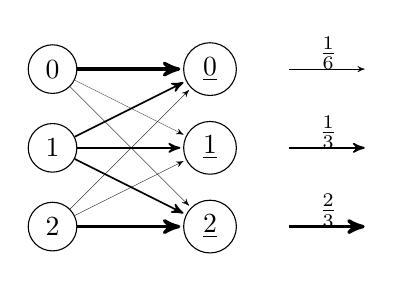
\begin{tikzpicture}[->,>=stealth',shorten >=1pt,auto,node
      distance=2cm,node/.style={circle,draw}]
      \node[node] (i0) at ( -2,  1) { $0$ };
      \node[node] (i1) at ( -2,  0) { $1$ };
      \node[node] (i2) at ( -2, -1) { $2$ };

      \node[node] (o0) at (  0,  1) { $\underline{0}$ };
      \node[node] (o1) at (  0,  0) { $\underline{1}$ };
      \node[node] (o2) at (  0, -1) { $\underline{2}$ };

      \hide{
      \node at (1.5,  1) {
        $
        \begin{array}{l}
          0(1),1(0),2(0)
        \end{array}
        $ };
      \node at (1.5,  0) {
        $
        \begin{array}{l}
          0(0),1(1),2(0)
        \end{array}
        $ };
      \node at (1.5, -1) {
        $
        \begin{array}{l}
          0(0),1(0),2(1)
        \end{array}
        $ };
      }

      \draw[->,very thick] (i0) -- (o0);   % 2/3
      \draw[->,ultra thin]  (i0) -- (o1);   % 1/6
      \draw[->,ultra thin]  (i0) -- (o2);   % 1/6

      \draw[->,semithick] (i1) -- (o0);               % 1/3
      \draw[->,semithick] (i1) -- (o1);               % 1/3
      \draw[->,semithick] (i1) -- (o2);               % 1/3

      \draw[->,ultra thin]  (i2) -- (o0);   % 1/6
      \draw[->,ultra thin]  (i2) -- (o1);   % 1/6
      \draw[->,very thick] (i2) -- (o2);   % 2/3

      \node at (1.5, 1.2) { $\frac{1}{6}$ };
      \draw[->,ultra thin] (1,  1) -- (2,  1);
      \node at (1.5, 0.2) { $\frac{1}{3}$ };
      \draw[->,semithick]  (1,  0) -- (2,  0);
      \node at (1.5,-0.8) { $\frac{2}{3}$ };
      \draw[->,very thick] (1, -1) -- (2, -1);
      
\hide{      
      \path
      (i0) edge node[above] { $\frac{2}{3}$ } (o0)
      (i0) edge node { $\frac{1}{6}$ } (o1)
      (i0) edge node[below] { $\frac{1}{6}$ } (o2)

      (i1) edge node[above] { $\frac{1}{3}$ } (o0)
      (i1) edge node { $\frac{1}{3}$ } (o1)
      (i1) edge node[below] { $\frac{1}{3}$ } (o2)

      (i2) edge node[above] { $\frac{1}{6}$ } (o0)
      (i2) edge node { $\frac{1}{6}$ } (o1)
      (i2) edge node[below] { $\frac{2}{3}$ } (o2)
      ;
    }
      \end{tikzpicture}
    }
  \caption{Truncated $\frac{1}{2}$-Geometric Mechanism}
  \label{figure:geometric-mechanism}
\end{figure}

\noindent
\textit{Example 1.}
To see how differential privacy works, let us consider the truncated
$\frac{1}{2}$-geometric mechanism
(Figure~\ref{figure:geometric-mechanism}). 
In the figure, the states $0$, $1$, and $2$ denote the number of
individuals contracting the disease; the states $\underline{0}$,
$\underline{1}$, $\underline{2}$ denote the outputs of the
mechanism. At the state $\underline{0}$, \textit{zero} is observed
with probability $1$ but \textit{one} and \textit{two} can never be 
observed. Similarly, the states $\underline{1}$ and $\underline{2}$
only observe \textit{one} and \textit{two} respectively. 
In the figure, thin arrows denote transitions with probability
$\frac{1}{6}$; medium arrows denote transitions with probability
$\frac{1}{3}$; thick arrows denote transitions with probability
$\frac{2}{3}$. For instance, the state $0$ can transit to the state
$\underline{0}$ with probability $\frac{2}{3}$ while it can transit to
the state $\underline{1}$ with probability $\frac{1}{6}$.

Let us consider a data set whose two members (including John) contract
the disease. Thus the number of individuals contracting the disease is
$2$. From the state $2$, we see the mechanism answers
\textit{zero}, \textit{one}, and \textit{two} with probabilities
$\frac{1}{6}$, $\frac{1}{6}$, and $\frac{2}{3}$ respectively. 
Suppose we replace John with an individual who does not contract
the disease. The number of individuals contracting the disease for the
new data set is $1$. From the state $1$, we see the mechanism answers
\textit{zero}, \textit{one}, and \textit{two} with the probability
$\frac{1}{3}$.

If an attacker queries the number of individuals contracting the
disease through the truncated $\frac{1}{2}$-geometric mechanism, 
he will get the answer \textit{two} with probability at least
$\frac{1}{3}$ regardless of John's record. The truncated
$\frac{1}{2}$-geometric mechanism is known to be
$\ln(2)$-differentially private. For any two similar data sets, the
mechanism always have similar output distributions. Information
revealed to attackers is therefore limited.

\noindent
\textit{Example 2.}
It is interesting to see when differential privacy may fail. Consider
a data set consisting of two family members and a contagious
disease. An attacker will immedidately infer the number of individuals
contracting the disease can only be $0$ or $2$. If none has contracted
the disease, the attacker observes \textit{zero}, \textit{one}, and
\textit{two} with probabilities $\frac{2}{3}$, $\frac{1}{6}$, and
$\frac{1}{6}$ respectively. If the two members have the disease, the
probabilities are $\frac{1}{6}$, $\frac{1}{6}$, and $\frac{2}{3}$
respectively. Note that it is $4 = \frac{2/3}{1/6}$ times more likely
to observe \textit{zero} when there is none contracting the disease
than there are two. Similarly, it is $4$ times more likely to observe
\textit{two} in the other case. Even though the
$\frac{1}{2}$-geometric mechanism is $\ln(2)$-differentially private,
it may reveal too much information \emph{when the attacker has prior
 knowledge about the data set and disease.}


\noindent
\textit{Example 3.}
Let us analyze the scenario in the previous example with the
Pufferfish privacy framework. Suppose the attacker knows that the data
set contains two family members and the disease is contagious. We
would like to compare the probabilities of observing \textit{zero}
when a member has contracted the disease or not. If a family member
has contracted the disease, the number of individuals contracting
the disease must be $2$ by the prior knowledge. The attacker thus
observes \textit{zero} with probability $\frac{1}{6}$.
If, on the other hand, a family member has not contracted
the disease, the number of individuals contracting the disease must be
$0$ by the prior knowledge. The attacker observes \textit{zero}
with probability $\frac{2}{3}$. The probabilities of observing
\textit{zero} are $\frac{1}{6}$ and $\frac{2}{3}$ when a family
has contracted the disease or not respectively. The
$\frac{1}{2}$-geometric mechanism does not satisfy 
$\ln(2)$-Pufferfish privacy. 

\noindent
\textit{Example 4.}
Prior knowledge does not necessarily lead to privacy leak. Consider a
non-contagious disease. An attacker may know that contracting the
disease is an independent event with probability $p$. Even though the
attacker does not know how many individuals have disease exactly, the
person can still infer that the number of individuals contracting the
disease is $0$, $1$, and $2$ with probabilities $(1-p)^2$, $2p(1-p)$,
and $p^2$ respectively. The prior knowledge can be easily formalized
by an information state in Figure~\ref{figure:geometric-mechanism}.
Consider the information
state where the probabilities at the states $0$, $1$, $2$,
$\underline{0}$, $\underline{1}$, and $\underline{2}$ are $(1-p)^2$,
$2p(1-p)$, $p^2$, $0$, $0$, and $0$ respectively.

Using the Pufferfish framework, we analyze the $\frac{1}{2}$-geometric
mechanism with the prior knowledge as follows. Assume the data set
contains John's record and John has contracted the disease. We would
like to compare probabilities of observations \textit{zero},
\textit{one}, and \textit{two} conditioned on the prior knowledge and
the presence/absence of John's record.

Suppose John's record is not in the data set. With the attacker's
prior knowledge, we see that the mechanism outputs \textit{zero} with
probability $(1-p)^2 \times \frac{2}{3} + 2p(1-p) \times \frac{1}{3} +
p^2 \times \frac{1}{6} = \frac{1}{6} p^2 - \frac{2}{3} p +
\frac{2}{3}$. Similarly, the mechanism outputs \textit{one} and
\textit{two} with probabilities $-\frac{1}{3} p^2 + \frac{1}{3} p +
\frac{1}{6}$ and $\frac{1}{6} p^2 + \frac{1}{3} p + \frac{1}{6}$
respectively.

Now suppose John's record is indeed in the data set. Since John has
the disease, the number of individuals contracting the disease cannot
be $0$. Conditioned on the prior knowledge, we have another
information state whose probabilities at the states $0$, $1$, $2$,
$\underline{0}$, $\underline{1}$, and $\underline{2}$ are $0$,
$\frac{2p(1-p)}{2p(1-p) + p^2} = \frac{2-2p}{2-p}$,
$\frac{p^2}{2p(1-p) + p^2} = \frac{p}{2-p}$, $0$, $0$, and $0$
respectively. From this information state, the mechanism outputs
\textit{zero}, \textit{one}, and \textit{two} with probabilities
$\frac{4-3p}{12-6p}$, $\frac{4-3p}{12-6p}$, and $\frac{2}{6-3p}$
respectively. Table~\ref{table:Pufferfish-geometric-mechanism}
summarizes observation probabilities.

\begin{table}
  \caption{Pufferfish Anlysis of $\frac{1}{2}$-Geometric Mechanism}
  \label{table:Pufferfish-geometric-mechanism}
  \centering
  \[
    \begin{array}{c|ccc}
      & \textit{zero} & \textit{one} & \textit{two} \\
      \hline
      \textmd{without John's record}
      & \frac{p^2 - 4p + 4}{6}
      & \frac{-2p^2 + 2p + 1}{6}
      & \frac{p^2 + 2p + 1}{6}
      \\

      \textmd{with John's record}
      & \frac{4-3p}{12-6p}
      & \frac{4-3p}{12-6p}
      & \frac{2}{6-3p}
    \end{array}
  \]
\end{table}

For observation \textit{zero}, it is not hard to check $\frac{1}{2}
\times \frac{4-3p}{12-6p} \leq \frac{p^2 - 4p + 4}{6} \leq 2 \times
\frac{4-3p}{12-6p}$ for any $0 \leq p \leq 1$. Similarly, we have
$\frac{1}{2} \times 
\frac{4-3p}{12-6p} \leq \frac{-2p^2 + 2p + 1}{6} \leq 2 \times
\frac{4-3p}{12-6p}$ and $\frac{1}{2} \times \frac{2}{6-3p} \leq
\frac{p^2 + 2p + 1}{6} \leq 2 \times \frac{2}{6-3p}$  for observations
\textit{one} and \textit{two} respectively. Therefore, the
$\frac{1}{2}$-geometric mechanism satisfies $\ln(2)$-Pufferfish
privacy when contracting the disease is \emph{independent}. 
 
In~\cite{KM:14:PFMPD}, it is shown that differential privacy is
subsumed by Pufferfish privacy (Theorem~6.1). This example is an
instance of the general theorem but formalized in hidden Markov
models. 

\noindent
\textit{Example 5.}
It is worth noting that independency of contracting disease is not
necessary for Pufferfish privacy. Let the probabilities of $0$, $1$,
and $2$ individuals contracting the disease are $p_0$, $p_1$, $p_2$
respectively. Then $p_0 + p_1 + p_2 = 1$. Moreover, the probabilities
of observing \textit{zero}, \textit{one}, and \textit{two} are
$\frac{2}{3} p_0 + \frac{1}{3} p_1 + \frac{1}{6} p_2$,
$\frac{1}{6} p_0 + \frac{1}{3} p_1 + \frac{1}{6} p_2$, and
$\frac{1}{6} p_0 + \frac{1}{3} p_1 + \frac{2}{3} p_2$ respectively.
Assume it is known that an individual in the data set has contracted
the disease. The probabilities of $0$, $1$, and $2$ individuals
contracting the disease become $0$, $\frac{p_1}{p_1 + p_2}$, and
$\frac{p_2}{p_1 + p_2}$ respectively. Consequently, the probabilities
of observing \textit{zero}, \textit{one}, and \emph{two} are
$\frac{\frac{1}{3}p_1 + \frac{1}{6}p_2}{p_1 + p_2}$,
$\frac{\frac{1}{3}p_1 + \frac{1}{6}p_2}{p_1 + p_2}$, and
$\frac{p_1 + 2p_2}{3(p_1 + p_2)}$ respectively. Choose $p_0 =
\frac{1}{2}$, $p_1 = p_2 = \frac{1}{4}$. For the observation
\textit{zero} we have, 
$\frac{1}{8} =
\frac{1}{2} \times \frac{\frac{1}{3}p_1 + \frac{1}{6}p_2}{p_1 + p_2}
\leq
\frac{11}{24} =
\frac{2}{3} p_0 + \frac{1}{3} p_1 + \frac{1}{6} p_2
\leq
{2} \times \frac{\frac{1}{3}p_1 + \frac{1}{6}p_2}{p_1 + p_2}
= \frac{1}{2}$.
Similarly, we have
$
\frac{1}{8} =
\frac{1}{2} \times \frac{\frac{1}{3}p_1 + \frac{1}{6}p_2}{p_1 + p_2}
\leq
\frac{5}{24} =
\frac{1}{6} p_0 + \frac{1}{3} p_1 + \frac{1}{6} p_2
\leq
2 \times \frac{\frac{1}{3}p_1 + \frac{1}{6}p_2}{p_1 + p_2}
= \frac{1}{2}$ for the observation \textit{one}. And
$
\frac{1}{4}
=
\frac{1}{2} \times \frac{p_1 + 2p_2}{3(p_1 + p_2)}
\leq
\frac{1}{3}
=
\frac{1}{6} p_0 + \frac{1}{3} p_1 + \frac{2}{3} p_2
\leq 
2 \times \frac{p_1 + 2p_2}{3(p_1 + p_2)}
= 1$ for the observation \textit{two}. In other words, the
$\frac{1}{2}$-geometric mechanism satisfies Pufferfish privacy for
attackers with the prior distribution $(\frac{1}{2}, \frac{1}{4},
\frac{1}{4})$ on the number of individuals contracting the disease.
Suppose the distribution $(\frac{1}{2}, \frac{1}{4},
\frac{1}{4})$ is binomial. There is $0 \leq p \leq 1$ such that
$(1-p)^2 = \frac{1}{2}$, $2p(1-p) = \frac{1}{4}$, and $p^2 =
\frac{1}{4}$. From $p^2 = \frac{1}{4}$ and $0 \leq p$, we have $p =
\frac{1}{2}$. But we would have $(1-p)^2 = \frac{1}{4} \neq
\frac{1}{2}$. Hence $(\frac{1}{2}, \frac{1}{4}, \frac{1}{4})$ is not
binomial. Even though the prior distribution is not derived by
independent contraction of the disease, $\frac{1}{2}$-geometric
mechanism does not reveal too much information. Independency of
contraction is not necessary for Pufferfish privacy on the geometric
mechanism. 



\section{Logic}
\label{section:logic}

\subsection{Syntax}

A \emph{state formula} $\phi$ is of the form
\[
  \top \ |\ 
  p \ |\ 
  \neg \phi \ |\ 
  \phi \wedge \phi \ |\ 
  \PJ{J} (\psi)
\]
where $\psi$ is a \emph{path formula} of the form
\[
  \X \psi \ |\ 
  \psi \until \psi \ |\ 
  \psi \until^{\leq n} \psi.
\]

\subsection{Semantics}

Let $M = (\Act, S, p, L)$ be an MDP, $s \in S$, and $\phi$ a PCTL
state formula. Define $M, s \models \phi$ as follows.

\[
\myPr{s}{K}{\phi} =
\Pr [ \{ \pi : K, \pi \models \psi \textmd{ with } \pi_0 = s \} ].
\]


\begin{eqnarray*}
  M, s \models \top\\
  M, s \models p  & \textmd{ if } &  p \in L(s)\\
  M, s \models \neg \phi  & \textmd{ if } &  M, s \not\models \phi\\
  M, s \models \phi \wedge \phi'
  & \textmd{ if } & M, s \models \phi \textmd{ and }
                    M, s \models \phi'\\
  M, s \models \PJ{J} \psi
  & \textmd{ if } &
  \myPr{s}{M_{\scheduler{S}}}{\psi} \in J
  \textmd{ for every scheduler } \scheduler{S}
\end{eqnarray*}

\begin{eqnarray*}
  K, \pi \models \X \psi
  & \textmd{ if } &
  K, \pi[1] \models \psi\\
  K, \pi \models \psi \until \psi'
  & \textmd{ if } &
  \textmd{there is a } j \geq 0 \textmd{ such that }
  K, \pi[j] \models \psi' \textmd{ and } \\
  & & K, \pi[k] \models \psi
      \textmd{ for every } 0 \leq k < j \\
  K, \pi \models \psi \until^{\leq n} \psi'
  & \textmd{ if } &
  \textmd{there is a } n \geq j \geq 0 \textmd{ such that }
  K, \pi[j] \models \psi' \textmd{ and } \\
  & & K, \pi[k] \models \psi \textmd{ for every } 0 \leq k < j
\end{eqnarray*}


Let $P = (M, \Obs, r)$ be a POMDP, $\info \in \info (S)$, and
$\phi$ a PCTL state formula. Define
\begin{eqnarray*}
  \myE{\info}{K}{\psi} = E_{\info} [K, \pi \models \psi
  \textmd{ with } \pi_0 = s].
\end{eqnarray*}
Define $P, \info \models \phi$ as follows.
\begin{eqnarray*}
  P, \info \models \top \\
  P, \info \models p & \textmd{ if } & \info \in \valueof{p}\\
  P, \info \models \neg \phi & \textmd{ if } & P, \info \not\models \phi\\
  P, \info \models \phi \wedge \phi' & \textmd{ if } &
       P, \info \models \phi \textmd{ and } P, \info \models \phi'\\
  P, \info \models \PJ{J} (\psi) & \textmd{ if } &
       \myE{\info}{M_{\scheduler{S}}}{\psi} \in J \\
  P, \info \models \dpriv{\epsilon}{\delta} (\psi) & \textmd{ if } &
       \myE{\info}{M_{\scheduler{S}}}{\psi} \leq e^{\epsilon}
       \myE{\info'}{M_{\scheduler{S}}}{\psi} + \delta \textmd{ and }\\
  &&   \myE{\info'}{M_{\scheduler{S}}}{\psi} \leq e^{\epsilon}
       \myE{\info}{M_{\scheduler{S}}}{\psi} + \delta \textmd{ for
     every } \info N \info'.
\end{eqnarray*}


\section{Examples}
\label{section:examples}


\begin{figure}
  \centering
  \resizebox{.6\columnwidth}{!}{
    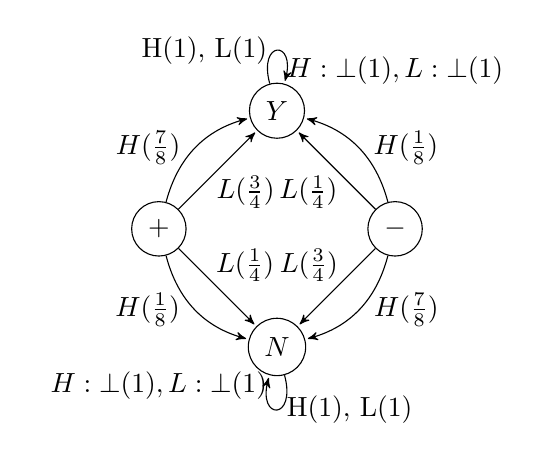
\begin{tikzpicture}[->,>=stealth',shorten >=1pt,auto,node
      distance=2cm,node/.style={circle,draw}]
      \node[node] (p) at ( -1.5,  0) { $+$ };
      \node[node] (n) at (  1.5,  0) { $-$ };
      \node[node] (Y) at (  0,  1.5) { $Y$ };
      \node[node] (N) at (  0, -1.5) { $N$ };

      \node at (1.5,  2) {
        $
        \begin{array}{l}
          H:\bot(1),L:\bot(1)
        \end{array}
        $ };
      \node at (-1.5, -2) { 
        $
        \begin{array}{l}
          H:\bot(1),L:\bot(1)
        \end{array}
        $ };

      \path
      (p) edge [bend left] node [above, left=2] { $H(\frac{7}{8})$ } (Y)
      (p) edge [bend right] node [below, left=2] { $H(\frac{1}{8})$ } (N)
      (p) edge node [below=8, right=-4] { $L(\frac{3}{4})$ } (Y)
      (p) edge node [above=8, right=-4] { $L(\frac{1}{4})$ } (N)
      (n) edge [bend right] node [above, right=2] { $H(\frac{1}{8})$ } (Y)
      (n) edge [bend left]node [below, right=2] { $H(\frac{7}{8})$ } (N)
      (n) edge node [below=8, left=-4] { $L(\frac{1}{4})$ } (Y)
      (n) edge node [above=8, left=-4] { $L(\frac{3}{4})$ } (N)

      (Y) edge [loop above] node [left] { H(1), L(1) } (Y)
      (N) edge [loop below] node [right] { H(1), L(1) } (N)
      ;
      \end{tikzpicture}
    }
  \caption{Survey Query 0}
  \label{figure:survey-0}
\end{figure}

Let $(\Pr (s = +), \Pr (s = Y), \Pr (s = N), \Pr (s = -))^T$ denote a
state distribution. In Figure~\ref{figure:survey-0}, we have
\[
  \begin{array}{rclcrcl}
    P^H & = &
      \left(
         \begin{array}{cccc}
           \  & \frac{7}{8} & \frac{1}{8} & \ \\
              &           1 &             &  \\
              &             &           1 &  \\
              & \frac{1}{8} & \frac{7}{8} &  
         \end{array}
\hide{              
         \begin{array}{cccc}
           0  & .875 & .125 & \ \\
              &    1 &      &  \\
              &      &    1 &  \\
              & .125 & .875 & 0 
         \end{array}
}
      \right)
    & 
    &
    P^L & = &
      \left(
         \begin{array}{cccc}
           \  & \frac{3}{4} & \frac{1}{4} & \ \\
              &           1 &             &   \\
              &             &           1 &   \\
              & \frac{1}{4} & \frac{3}{4} &   
         \end{array}
\hide{
         \begin{array}{cccc}
           0  & .75 & .25 & \ \\
              &   1 &     &   \\
              &     &   1 &   \\
              & .25 & .75 & 0
         \end{array}
}
      \right)
  \end{array}
\]
and
\[
  \begin{array}{rclcrcl}
    O^H (\bot) & = &
      \left(
         \begin{array}{cccc}
           0 & \ & \ & \  \\
             & 1 &   &    \\
             &   & 1 &    \\
             &   &   &  0 
         \end{array}
      \right)
    &&
    O^L (\bot) & = &
      \left(
         \begin{array}{cccc}
           0 & \ & \ & \  \\
             & 1 &   &    \\
             &   & 1 &    \\
             &   &   &  0 
         \end{array}
      \right)
  \end{array}
\]
Consider the state distribution $(\frac{1}{2}, 0, 0, \frac{1}{2})^T$.
Let $a:\omega$ denote that $\omega$ is observed after $a$. We have
\[
  (\frac{1}{2}, 0, 0, \frac{1}{2})^T
  \overset{H:\bot}{\longrightarrow}
  (0, \frac{1}{2}, \frac{1}{2}, 0)^T
  \overset{H:\bot}{\longrightarrow}
  (0, \frac{1}{2}, \frac{1}{2}, 0)^T.
\]
Now consider the probability of reaching the state $Y$ in one
action. We compute
\[
  \Gamma_2 = \{ (0, 1, 0, 0)^T \}
  \textmd{ and }
  \Gamma_1 = \{ (\frac{7}{8}, 1, 0, \frac{1}{8})^T (H),
                (\frac{3}{4}, 1, 0, \frac{1}{4})^T (L) \}.
\]
That is, for the state distribution $(\frac{1}{2}, 0, 0,
\frac{1}{2})^T$, the probability of reaching $Y$ is $0.5$ by taking
either action. For
the state distribution $(1, 0, 0, 0)^T$, the maximal probability of
reaching $Y$ becomes $\frac{7}{8}$ by taking the action $H$.


\begin{figure}
  \centering
  \resizebox{.6\columnwidth}{!}{
    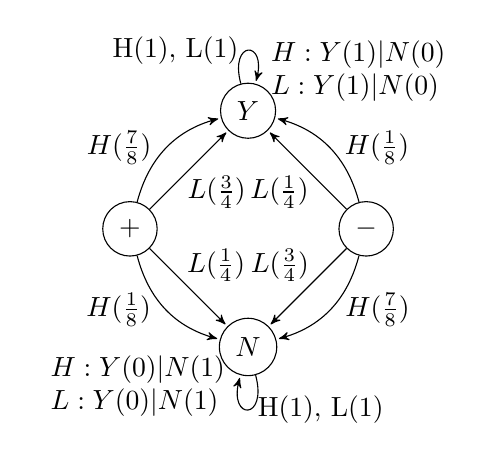
\begin{tikzpicture}[->,>=stealth',shorten >=1pt,auto,node
      distance=2cm,node/.style={circle,draw}]
      \node[node] (p) at ( -1.5,  0) { $+$ };
      \node[node] (n) at (  1.5,  0) { $-$ };
      \node[node] (Y) at (  0,  1.5) { $Y$ };
      \node[node] (N) at (  0, -1.5) { $N$ };

      \node at (1.4,  2) {
        $
        \begin{array}{l}
          H:Y(1)|N(0)\\L:Y(1)|N(0)          
        \end{array}
        $ };
      \node at (-1.4, -2) { 
        $
        \begin{array}{l}
          H:Y(0)|N(1)\\L:Y(0)|N(1)          
        \end{array}
        $ };

      \path
      (p) edge [bend left] node [above, left=2] { $H(\frac{7}{8})$ } (Y)
      (p) edge [bend right] node [below, left=2] { $H(\frac{1}{8})$ } (N)
      (p) edge node [below=8, right=-4] { $L(\frac{3}{4})$ } (Y)
      (p) edge node [above=8, right=-4] { $L(\frac{1}{4})$ } (N)
      (n) edge [bend right] node [above, right=2] { $H(\frac{1}{8})$ } (Y)
      (n) edge [bend left]node [below, right=2] { $H(\frac{7}{8})$ } (N)
      (n) edge node [below=8, left=-4] { $L(\frac{1}{4})$ } (Y)
      (n) edge node [above=8, left=-4] { $L(\frac{3}{4})$ } (N)

      (Y) edge [loop above] node [left] { H(1), L(1) } (Y)
      (N) edge [loop below] node [right] { H(1), L(1) } (N)
      ;
      \end{tikzpicture}
    }
  \caption{Survey Query 1}
  \label{figure:survey-1}
\end{figure}

Let $(\Pr (s = +), \Pr (s = Y), \Pr (s = N), \Pr (s = -))^T$ denote a
state distribution. In Figure~\ref{figure:survey-1}, we have
\[
  \begin{array}{rclcrcl}
    P^H & = &
      \left(
         \begin{array}{cccc}
           \  & \frac{7}{8} & \frac{1}{8} & \ \\
              &           1 &             &  \\
              &             &           1 &  \\
              & \frac{1}{8} & \frac{7}{8} &  
         \end{array}
      \right)
    & 
    &
    P^L & = &
      \left(
         \begin{array}{cccc}
           \  & \frac{3}{4} & \frac{1}{4} & \ \\
              &           1 &             &   \\
              &             &           1 &   \\
              & \frac{1}{4} & \frac{3}{4} &   
         \end{array}
      \right)
  \end{array}
\]
and
\[
  \begin{array}{rclcrclcrclcrcl}
    O^H (Y) & = &
      \left(
         \begin{array}{cccc}
           0 & \ & \ & \  \\
             & 1 &   &    \\
             &   & 0 &    \\
             &   &   &  0 
         \end{array}
      \right)
    &&
    O^H (N) & = &
      \left(
         \begin{array}{cccc}
           0 & \ & \ & \  \\
             & 0 &   &    \\
             &   & 1 &    \\
             &   &   &  0 
         \end{array}
      \right)
    &&
    O^L (Y) & = &
      \left(
         \begin{array}{cccc}
           0 & \ & \ & \  \\
             & 1 &   &    \\
             &   & 0 &    \\
             &   &   &  0 
         \end{array}
      \right)
    &&
    O^L (N) & = &
      \left(
         \begin{array}{cccc}
           0 & \ & \ & \  \\
             & 0 &   &    \\
             &   & 1 &    \\
             &   &   &  0 
         \end{array}
      \right)
  \end{array}
\]
Consider the state distribution $(\frac{1}{2}, 0, 0, \frac{1}{2})^T$.
Let $a:\omega$ denote that $\omega$ is observed after $a$. We have
\[
  (\frac{1}{2}, 0, 0, \frac{1}{2})^T
  \overset{H:Y}{\longrightarrow}
  (0, 1, 0, 0)^T
  \overset{H:Y}{\longrightarrow}
  (0, 1, 0, 0)^T.
\]
Now consider the probability of reaching the state $Y$ in one
action. We compute
\[
  \Gamma_2 = \{ (0, 1, 0, 0)^T \}
  \textmd{ and }
  \Gamma_1 = \{ (\frac{7}{8}, 1, 0, \frac{1}{8})^T (H),
                (\frac{3}{4}, 1, 0, \frac{1}{4})^T (L) \}.
\]
That is, for the state distribution $(\frac{1}{2}, 0, 0,
\frac{1}{2})^T$, the probability of reaching $Y$ is $0.5$ by
taking either action. For
the state distribution $(1, 0, 0, 0)^T$, the maximal probability of
reaching $Y$ becomes $\frac{7}{8}$ by taking the action $H$.

\begin{figure}
  \centering
  \resizebox{.9\columnwidth}{!}{
    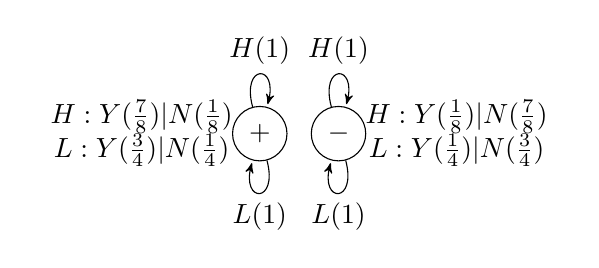
\begin{tikzpicture}[->,>=stealth',shorten >=1pt,auto,node
      distance=2cm,node/.style={circle,draw}]
      \node[node] (p) at ( -.5,  0) { $+$ };
      \node[node] (n) at (  .5,  0) { $-$ };

      \node at (-2, 0) {
        $
        \begin{array}{c}
          H:Y(\frac{7}{8})|N(\frac{1}{8})\\
          L:Y(\frac{3}{4})|N(\frac{1}{4})
        \end{array}
        $
      };
      \node at ( 2, 0) {
        $
        \begin{array}{c}
          H:Y(\frac{1}{8})|N(\frac{7}{8})\\
          L:Y(\frac{1}{4})|N(\frac{3}{4})
        \end{array}
        $
      };

      \path
      (p) edge [loop above] node { $H(1)$ } (p)
      (p) edge [loop below] node { $L(1)$ } (p)
      (n) edge [loop above] node { $H(1)$ } (n)
      (n) edge [loop below] node { $L(1)$ } (n)
      ;
      \end{tikzpicture}
    }
  \caption{Survey Query 2}
  \label{figure:survey-2}
\end{figure}

For Figure~\ref{figure:survey-2}, we have
\[
  \begin{array}{rcccl}
    P^H & = &
      \left(
         \begin{array}{cc}
           1 & \ \\
             & 1 
         \end{array}
      \right)
    & = & P^L
  \end{array}
\]
and
\[
  \begin{array}{rclcrclcrclcrcl}
    O^H (Y) & = &
      \left(
         \begin{array}{cc}
           \frac{7}{8} & \\
                       & \frac{1}{8} 
         \end{array}
      \right)
    &&
    O^H (N) & = &
      \left(
         \begin{array}{cc}
           \frac{1}{8} & \\
                       & \frac{7}{8} 
         \end{array}
      \right)
    &&
    O^L (Y) & = &
      \left(
         \begin{array}{cc}
           \frac{3}{4} & \\
                       & \frac{1}{4} 
         \end{array}
      \right)
    &&
    O^L (N) & = &
      \left(
         \begin{array}{cc}
           \frac{1}{4} & \\
                       & \frac{3}{4} 
         \end{array}
      \right)
  \end{array}
\]
Consider the state distriution $(\frac{1}{2}, \frac{1}{2})^T$. We have
\[
  (\frac{1}{2}, \frac{1}{2})^T
  \overset{H:Y}{\longrightarrow}
  (\frac{7}{8}, \frac{1}{8})^T
  \overset{H:Y}{\longrightarrow}
  (\frac{49}{50}, \frac{1}{50})^T.
\]
Moreover, let us compute the maximal expectation of reaching $+$ in
one action.
\[
  \Gamma_2 = \{ (1, 0)^T \} \textmd{ and }
  \Gamma_1 = \{ (1, 0)^T \}.
\]
From the state distriution $(\frac{1}{2}, \frac{1}{2})^T$, the maximal
expectation of reaching $+$ is hence $0.5$. This is expected since no
action can change the current state. If the probability of at state
$+$ is $0.5$ \emph{a priori}, the probability of reaching $+$ after
one action is again $0.5$ regardless of actions and observations.


\bibliographystyle{splncs03}
\bibliography{refs}

\end{document}
